\pagebreak
\chapter{Interfaccia del file system}\label{file system}
In questo capitolo ci occupiamo del \textit{file system}, ovvero metodo utilizzato dai sistemi operativi per gestire le memorie secondarie, in particolare i \textit{files}. Definiremo quindi il concetto di file e i metodi per accedervi. In secondo luogo si discuteremo di alcune nozioni delle quali sentiamo parlare tutti i giorni come \textit{folder} o \textit{directory} andando a vedere che cosa queste rappresentino nella pratica. Faremo poi alcune considerazioni riguardo la protezione.

\section{Concetto di file}
Partiamo dall'inizio: che cos'è un file? Un file è uno spazio di indirizzi logici contigui dove all'interno si possono scrivere o leggere dei dati. Tali dati possono essere numerici, binari, dei caratteri oppure possono essere dei particolari dati che corrispondono ad un effettivo file eseguibile o programma il quale potrà essere caricato in memoria ed eseguito dal processore.

Spesso, sopratutto nei sistemi Windows, i files sono identificati da un'\textbf{estensione} la quale agevola l'interpretazione del contenuto del file ma non è strettamente necessaria per il suo funzionamento. Generalmente è una sequenza di tre o quattro caratteri che viene separata dal nome del file da un punto. Estensioni tipiche in Windows sono \texttt{.exe .com} se si parla di una file eseguibile, \texttt{.obj .o} è un file compilato prima di essere linkato oppure \texttt{.txt .doc} per i documenti.

\subsection{Attributi e operazioni}\label{operazioni files}
Osserviamo inoltre che ogni file possiede delle proprietà, o \textbf{attributi}. Tipicamente questi attributi sono visualizzabili attraverso la sezione "Proprietà" del file oppure attraverso il terminale. Il \textbf{nome} è l'unica informazione leggibile dall'uomo e non è necessariamente univoco; l'\textbf{identificatore} invece è univoco (può essere un numero o un codice) e serve per distinguere ogni file precisamente all'interno del disco; il \textbf{tipo} indica il tipo di file (eseguibile, documento, etc) e inoltre segnala se tale file è supportato dal sistema operativo\footnote{Un eseguibile Windows non può infatti essere eseguito da un dispositivo Linux o UNIX.}; la \textbf{locazione} possiede informazioni sulla posizione fisica e logica del file sulla periferica; la \textbf{dimensione} indica lo spazio che occupa il file e la \textbf{protezione} fornisce informazioni che riguardano l'accesso in lettura/scrittura al file.

Normalmente queste informazioni sono contenute in una struttura chiamata \textit{directory} (vedi paragrafo \ref{directory}) la quale è mantenuta su disco e caratterizza il file system. 

I file supportano, ovviamente, diverse operazioni le quali sono generalmente fornite tramite \textbf{system calls}. Prima tra tutte è la \textbf{creazione} di un file seguita dalla \textbf{lettura} e la \textbf{scrittura} ad una determinata posizione del file. È inoltre possibile \textbf{riposizionare} il puntatore nel file: se lo si pensa come un array corrisponderebbe a puntare ad un altro indice. È consenta anche la \textbf{cancellazione} e il \textbf{troncamento}. Infine sono naturalmente presenti operazioni per \textbf{aprire} (in lettura/scrittura o entrambe) e \textbf{chiudere} il file.

% 
\subsection{Files aperti e file \textit{locking}}
Ogni volta che un file viene aperto il sistema operativo tiene traccia di questa apertura in una tabella apposita: l'\textbf{open-file table}. È anche presente un \textbf{file pointer} che indica dove andare ad operare nel file una volta che questo vine aperto. Tutte le volte che un file viene aperto, viene incrementato il contatore \textbf{file-open count}: questo valore non è altro che il numero di processi che hanno aperto quel file in particolare. Una volta che il processo è terminato e il file deve essere chiuso è necessario controllare che tutti i processi lo abbiano effettivamente chiuso al fine di rimuoverlo dalla \textit{open-file table}. La \textbf{disk location} è una cache che tiene temporaneamente i dati per fornire un accesso più veloce: ogni volta che si legge o scrive sul file non si fa direttamente su disco ma su questa cache.

Così come discusso nella sincronizzazione tra processi (vedi capitolo \ref{sincronizzazione}) dove sono presenti i \textbf{lock}, utili per accedere ad una sezione critica di un processo senza avere interferenza da altri processi, anche nel caso dei file è possibile utilizzare dei \textit{lock} volti a garantire l'accesso esclusivo di un processo ad un file. La soluazione consigliata è quella di utilizzare un \textit{lock} esclusivo in scrittura e uno condiviso in lettura del file. In questo modo si garantisce che un file sia scritto solo da un processo alla volta oppure che venga letto da più processi contemporaneamente.

I sistemi operativi possono implementare versioni più avanzate di questi lucchetti, alcuni di questi che sono obbligatori, ovvero che bloccano l'accesso a file e nessun altro può accedervi, altri invece sono così detti "suggeriti", dove la scelta di accesso è lasciata al sistema operativo.

% 
\subsection{Struttura del file}
La struttura del file può essere pensata come una sequenza logica contigua di byte in memoria. Ciò nonostante tale sequenza può concettualmente rappresentare delle strutture dati che non sono dei semplici array ma possono essere, per esempio, degli alberi. Questa struttura è dettata dal tipo di file o tipo di applicazione.

%
\section{Metodi di accesso}
Una caratteristica importante del file è che ha una dimensione fissa, a differenza dei dati in memoria: questo semplifica sicuramente l'accesso al file. Due sono i metodi per l'accesso: uno è sequenziale l'altro invece è diretto (o \textit{random}).

\subsection{Accesso sequenziale}
La tecnica di accesso sequenziale implica lo scorrimento del puntatore lungo tutto il file. Al fine di accedere ad un dato che si trova prima rispetto al puntatore è necessario fare una \textbf{reset} del puntatore per poi scorrere nuovamente il file (figura \ref{fig:accesso sequenziale}).
\begin{figure}[h]
    \centering
    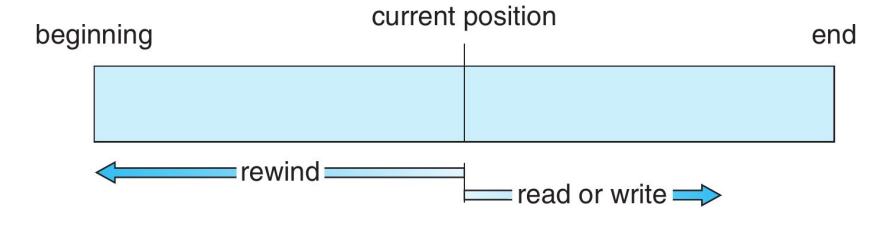
\includegraphics[width = .5\textwidth]{../res/imgs/file system interface/accesso sequenziale.png}
    \caption{L'accesso sequenziale ad un file.}
    \label{fig:accesso sequenziale}
\end{figure}
Questo è un algoritmo di accesso molto semplice, vagamente simile all'algoritmo scan per quanto riguarda i dischi (vedi paragrafo \ref{scan}).

Avremo quindi delle istruzioni per leggere o scrivere il byte o la \textit{word} successiva e un'istruzione per effettuare l'operazione di reset

% 
\subsection{Accesso diretto}
Quando parliamo di un accesso diretto, o \textbf{random}, parliamo di meccanismo più complesso sia dal punto di vista software che hardware che però garantisce una velocità maggiore. 

In questo caso abbiamo invece delle istruzioni pù sofisticate in quanto è possibile esplicitare l'\textbf{n}-esimo byte da leggere o scrivere. È inoltre possibile simulare un accesso di tipo sequenziale utilizzando istruzioni come \texttt{read next} oppure \texttt{write next}.

% 
\section{Struttura della directory}\label{directory}
Fino ad ora abbiamo parlato di file come elemento base per lavorare e memorizzare dati su memorie secondarie. Ora invece saliamo di un livello di astrazione e andiamo ad occuparci di che cos'è e come è strutturata una directory.

La directory è una struttura che supporta l'utilizzo dei files e  consente l'effettivo accesso al file. Possiamo dire, in altre parole, che è una \textbf{collezione di puntatori} o nodi (figura \ref{fig:struttura directory}) che contengono informazioni dei files.

\begin{figure}[h]
    \centering
    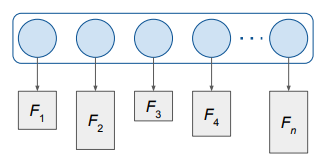
\includegraphics[width =.45\textwidth]{../res/imgs/file system interface/struttura directory.png}
    \caption{La struttura concettuale-minimale di una directory.}
    \label{fig:struttura directory}
\end{figure}

Così come è possibile effettuare delle operazioni su file (\ref{operazioni files}), anche la directory supporta delel operazioni. Tra queste ci sono la \textbf{ricerca} di un file, \textbf{creare un nodo} che punta ad un file, \textbf{eliminare} un file, \textbf{listare} il contenuto della directory oppure rinominare e attraversa il file system. La directory garantisce l'\textbf{accesso efficiente} ai files (1), gestisce il modo in cui tali files possono essere nominati (2) in modo tale che due utenti possono fare riferimento allo stesso file utilizzando nomi diversi. Si possono inoltre raggruppare i files (3) in base alle loro proprietà e al loro utilizzo. Questi tre punti saranno utilizzati in seguito per comparare le diverse strutture.

\subsection{Directory a uno e due livelli}
L'approccio più semplice per rappresentare la struttura di una directory è attraverso una singola struttura che contiene un puntatore a tutti i files presenti sul disco (vedi figura \ref{fig:single-level dir}).
\begin{figure}[h]
    \centering
    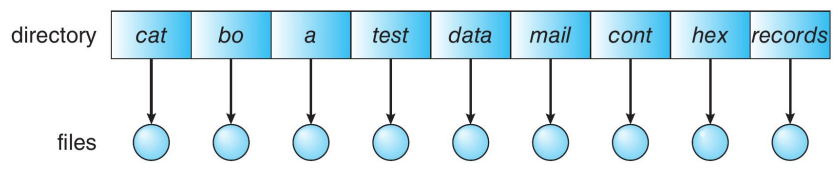
\includegraphics[width = .7\textwidth]{../res/imgs/file system interface/single-level dir.png}
    \caption{Struttura di una direcotory a livello singolo.}
    \label{fig:single-level dir}
\end{figure}
Per quanto banale, per determinati sistemi, come quelli \textit{embedded}\footnote{I sistemi embedded sono sistemi integrati. L'esempio più banale è il controllore di un cancello elettronico oppure il processore di una lavatrice.} che hanno a disposizione poche risorse è una struttura più che adeguata. Questa struttura si traduce in tutti gli effetti in una tabella che contiene un puntatore con relazione uno a uno da nome alla posizione del file sul disco. Con questa struttura non siamo ovviamente in grado di soddisfare i 3 punti elencati in precedenza.

Per riuscire a soddisfare i 3 punti precedenti è necessario aumentare il livello di complessità: una soluzione sensata è quindi quella di aggiungere un ulteriore livello (figura \ref{fig:two-level dir}). Questa rappresentazione torna nel momento in cui dobbiamo rappresentare un sistema multiutente dove è presente una \textit{master file directory} che contiene il nome di tutti gli utenti, ognuno dei quali ha una propria directory personale.
\begin{figure}[h]
    \centering
    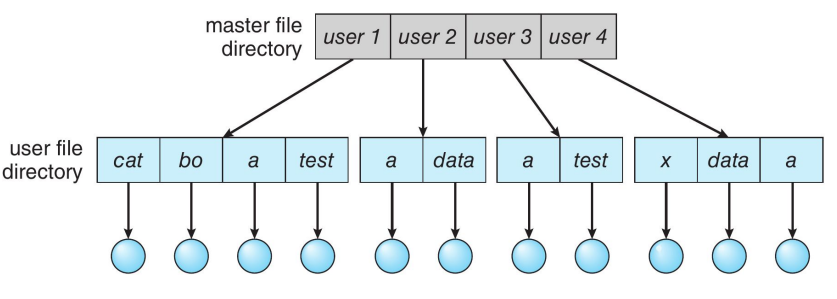
\includegraphics[width = .65\textwidth]{../res/imgs/file system interface/two-level dir.png}
    \caption{Struttura di una directory a due livello}
    \label{fig:two-level dir}
\end{figure}
In questo modo è possibile risolvere il problema del \textbf{naming}, ovvero avere file con lo stesso nome per utenti diversi, abbiamo una ricerca più efficiente ma comunque il \textbf{raggruppamento} non è ancora possibile.

% 
\subsection{Directory strutturata ad albero}
\begin{figure}[h]
    \centering
    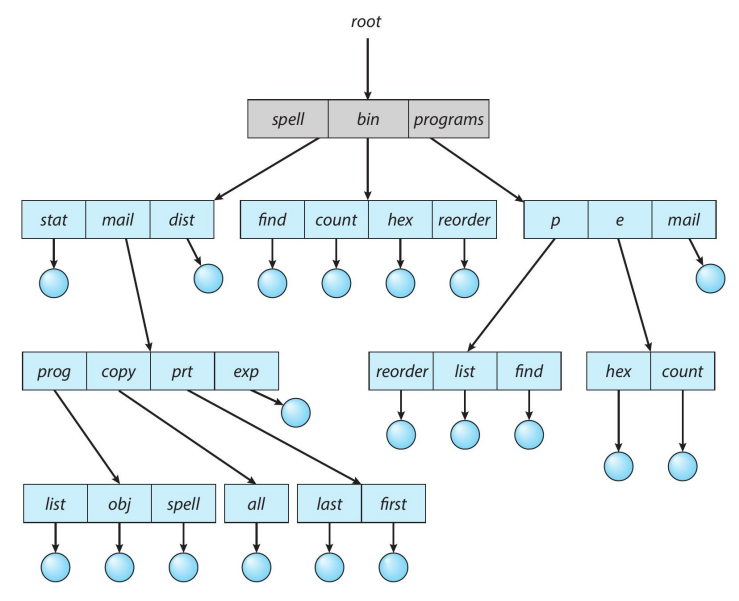
\includegraphics[width = .6\textwidth]{../res/imgs/file system interface/tree-structured dir.png}
    \caption{Rappresentazione di una directory strutturata ad albero.}
    \label{fig:tree-structured dir}
\end{figure}
Arriviamo quindi ad una struttura di directory che si avvicina molto a quelle che sono le directory di sistemi operativi moderni con cui normalmente lavoriamo. Queste presentano un numero potenzialmente infinito di strutture a diversi livelli: ecco che si ha una \textbf{struttura ad albero}. All'interno di tale struttura un bit che indica se la struttura è un file o una directory. 

Il percorso per l'accesso ad un file può essere specificato in modo relativo o assoluto. Nel primo caso si specificano le operazioni da fare dalla posizione corrente mentre nel secondo caso è riferito solo alla \textit{root}, ovvero il nodo principale da cui è strutturato il file system.

\subsection{Problema dei cicli}
Nel lavorare con questo tipo di strutture si può incorrere nel \textbf{problema} della possibile creazione di \textbf{cicli}. Per esempio se abbiano a che fare con una struttura ad albero e creiamo un \textbf{link} a directory o files possiamo avere a che fare con cicli. Osserviamo la figura \ref{fig:acyclic-graph dir} possiamo notare che due sotto-directory diverse puntano entrambe ad un file che si trova nella directory \texttt{list}. Questo ciclo deve essere gestito dal sistema operativo.
\begin{figure}[h]
    \centering
    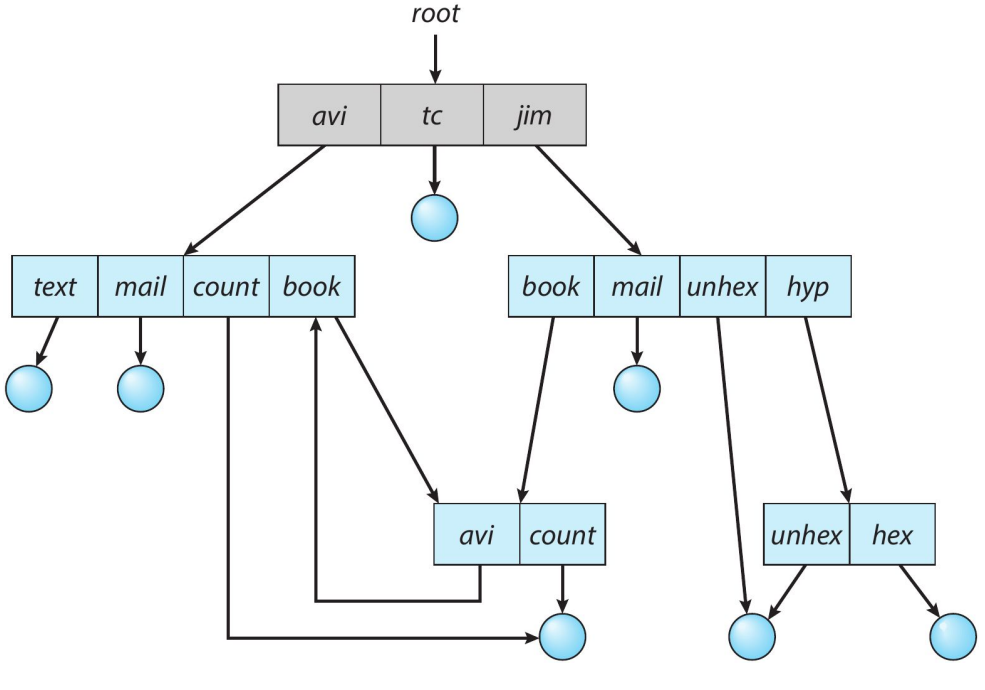
\includegraphics[width = .5\textwidth]{../res/imgs/file system interface/general graph dir.png}
    \caption{Rappresentazione generica di una directory.}
    \label{fig:acyclic-graph dir}
\end{figure}
Se infatti eliminiamo l'intera directory \texttt{avi} la directory \texttt{jim/book} punterà ad una directory inesistente in quanto eliminata: stiamo parlando dei \textbf{dangling pointers}. Come possiamo risolvere questa soluzione? Ci sono diversi modi. Primo tra tutti è l'eliminazione di tutti i link oppure, il file viene eliminato solo nel momento in cui tutti i riferimenti a tale file sono rimossi\footnote{Molto simile al concetto dello \texttt{shared\_pointer} di C++.}.

Ci sono quindi diversi modi per gestire i cicli all'interro di queste strutture.
\vspace{-5px}
\begin{enumerate}
\setlength{\itemsep}{-.15 em}
    \item Evitare i cicli: ogni volta che si crea un riferimento che genera un ciclo, proibirne la creazione;
    \item Ad ogni link creato, verificare se viene creato un ciclo gestibile oppure se può creare dei problemi;
    \item Permettere la creazione di cicli, ma evitare loop infiniti di ricerca di file attraverso qualche contatore che impedisca la ricerca ciclica di un file;
    \item Attraverso la \textbf{garbage collection}: viene eseguito un processo a parte periodicamente che elimina i \textit{dangling pointers}.
\end{enumerate}

% 
\subsection{Disco}
Il disco rigido è organizzato e strutturato per fornire, ovviamente, la possibilità di immagazzinare files. Normalmente è diviso in \textbf{partizioni} che possono essere di diverso tipo a seconda dell'uso. Ci possono essere delle partizioni di tipo \textbf{RAID} (vedi paragrafo \todo{riferimento RAID}), di tipo \textbf{raw}, cioè che possono essere utilizzate direttamente da un database che gestisce a modo suo l'informazione, di tipo \textbf{swap} che permettono un accesso veloce (come cache) o anche \textbf{formattate} con un determinato file system e di conseguenza inizializzati con una particolare struttura che varia a seconda del sistema operativo o a seconda dell'utilizzo che ne vogliamo fare\footnote{Per esempio, nei sistemi Windows abbiamo partizioni di tipo NTFS.}.

Normalmente la partizione di disco che contiene il file system viene chiamata anche \textit{volume}. All'interno di esso troviamo una \textit{device directory}, ovvero una directory principale che contiene le informazioni generali sul contenuto del volume.

% 
\section{Protezione}\label{protection}
Come sui file c'è l'attributo per la loro protezione, anche nel caso delle directory emerge la questione di come proteggere sia il contenuto del file che dell'intera directory. Uno dei primi obiettivi che è necessario raggiungere è quello di riuscire a proteggere i files o le directory create dell'utente. Si vorrebbe che l'utente proprietario di un determinato file o directory abbia un accesso privilegiato rispetto ad altri utenti. Per gestire la proprietà del file è quindi necessario gestire azioni in lettura, scrittura, esecuzione, rimozione, aggiunta o \textit{list}.

\subsection{Access list in Unix/Linux}\label{permissions}
Nei sistemi operativi Unix/Linux tipicamente si identificano tre tipi di accesso: \textit{read} (\texttt{R}), \textit{write} (\texttt{W}) ed \textit{execute} (\texttt{X}); e tre classi di utente: \textit{owner}, gruppo e una classe pubblica. Per gestire gli accessi si usa quindi la terna \texttt{RWX} binaria. Per esempio, se all'\textit{owner} è assegnato \texttt{111 = 7} (attraverso il comando \texttt{chmod}) ha accesso sia in lettura, che in scrittura che in esecuzione del file questo perché i 3 bit che rappresentano \texttt{RWX} sono tutti e 3 ad 1. Se invece all'accesso pubblico assegniamo \texttt{100 = 4}, questi avranno accesso solo in lettura.
